\chapter{КОНСТРУКТОРСКАЯ ЧАСТЬ}

В данном разделе будут представлены этапы проектирования системы. Будут описаны таблицы и их атрибуты, проектируемой базы данных. Будет разработана ER-диаграмма базы данных. Будет разработан алгоритм преобразования информации о жанрах игры из строчного представления в xml формат. Будет разработана UML диаграмма компонента бизнес-логики и компонента доступа к базе данных.

\section{Описание таблиц разрабатываемой базы данных}

Согласно ER-диаграмме, показанной на рисунке~\ref{img:er}, в базе данных выделены и реализованы следующие таблицы:

\begin{enumerate}
	\item таблица с играми Games;
	\item таблица с временными отметками TimeRecords;
	\item таблица с отзывами Reviews;
	\item таблица с пользователями Users;
	\item таблица с платформами Platforms;
	\item таблица связка платформ и игр GamePlatform;
\end{enumerate}

На рисунке~\ref{fig:erbd} представлена ER-диаграмма базы данных.

\begin{figure}[H]
	\centering
	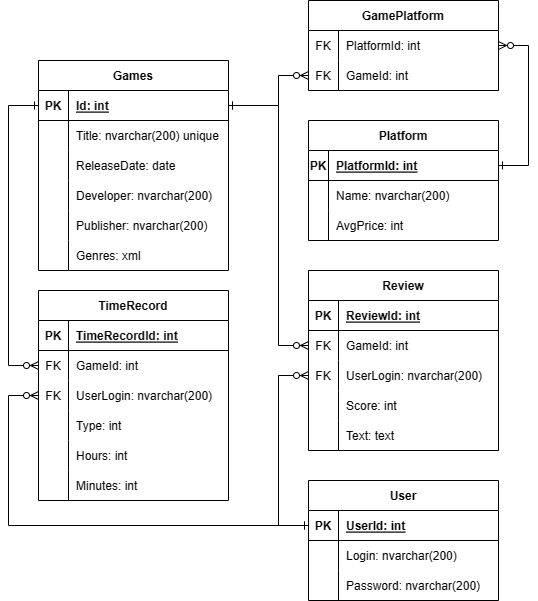
\includegraphics[width=0.8\linewidth]{../imgs/er_bd}
	\captionsetup{justification=centering}
	\caption{Диаграмма сущность-связь базы данных}
	\label{fig:erbd}
\end{figure}

В таблице Games, которая содержит информацию об играх, представлены следующие атрибуты:

\begin{enumerate}
	\item Id --- идентификатор игры, первичный ключ, int;
	\item Title --- уникальное название игры, string;
	\item ReleaseDate --- дата выхода игры, date;
	\item Developer --- разработчик игры, string;
	\item Publisher --- издатель, string;
	\item Genres --- жанры, xml.
\end{enumerate}

В таблице Platforms, которая содержит информацию о платформах, представлены следующие атрибуты:

\begin{enumerate}
	\item Id --- идентификатор платформы, первичный ключ, int;
	\item Name --- уникальное название платформы, string;
	\item AvgPrice --- средняя цена платформы, int.
\end{enumerate}

В таблице GamePlatform, которая содержит информацию о связи игр и платформ, представлены следующие атрибуты:

\begin{enumerate}
	\item GameId --- идентификатор игры, int;
	\item PlatformId --- идентификатор платформы, int.
\end{enumerate}

В таблице TimeRecords, которая содержит информацию о временных отметках на игре, представлены следующие атрибуты:

\begin{enumerate}
	\item Id --- идентификатор, int;
	\item GameId --- идентификатор игры, int;
	\item UserLogin --- имя пользователя который оставил эту отметку, string;
	\item Hours ---  количество полных часов потраченных на прохождение игры, int;
	\item Minutes --- количество полных минут потраченных на прохождение игры, int;
	\item Type --- тип прохождения, int. 
\end{enumerate}

В таблице Reviews, которая содержит информацию об отзывах, представлены следующие атрибуты:

\begin{enumerate}
	\item Id --- идентификатор, int;
	\item GameId --- идентификатор игры на которую оставлен отзыв;
	\item UserLogin --- имя пользователя оставившего отзыв, string;
	\item Text --- текст отзыва, string;
	\item PublicationDate --- дата публикации отзыва, date.
\end{enumerate}

В таблице Users, которая содержит информацию о пользователях, представлены следующие атрибуты:

\begin{enumerate}
	\item Login --- имя пользователя, string;
	\item Password --- пароль, string.
\end{enumerate}

\section{Схема алгоритма преобразования строки в xml формат}

На рисунке~\ref{fig:xmltransform} представлена преобразования строки в xml формат. Сначала алгоритм преобразует данные из одной строки, в которой содержится информация о жанрах, в массив строк, каждая из которых описывает отдельный жанр. Затем каждый из элементов полученного массива будет записан в строку в xml формате. Информация в xml формате может быть успешно вставлена в таблицу.

\begin{figure}[H]
	\centering
	\captionsetup{justification=centering}
	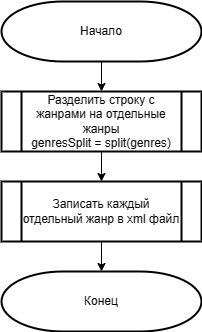
\includegraphics{../imgs/xmlTransform}
	\caption{Схема алгоритма преобразования строки в xml формат}
	\label{fig:xmltransform}
\end{figure}

\section{Диаграмма классов приложения}

Диаграмма классов компонента доступа к базе данных и компонента бизнес-логики показана на рисунке~\ref{fig:uml}. 

Доступ к компоненту бизнес-логики осуществляется через интерфейсы сервисов. Доступ к компоненту базы данных осуществляется через Repository классы. Компонент бизнес-логики связан с компонентом доступа к базе данных через Repository интерфейсы. Таким образом, бизнес-логика не зависит от реализации компонента доступа к базе данных. 

\begin{figure}[H]
	\centering
	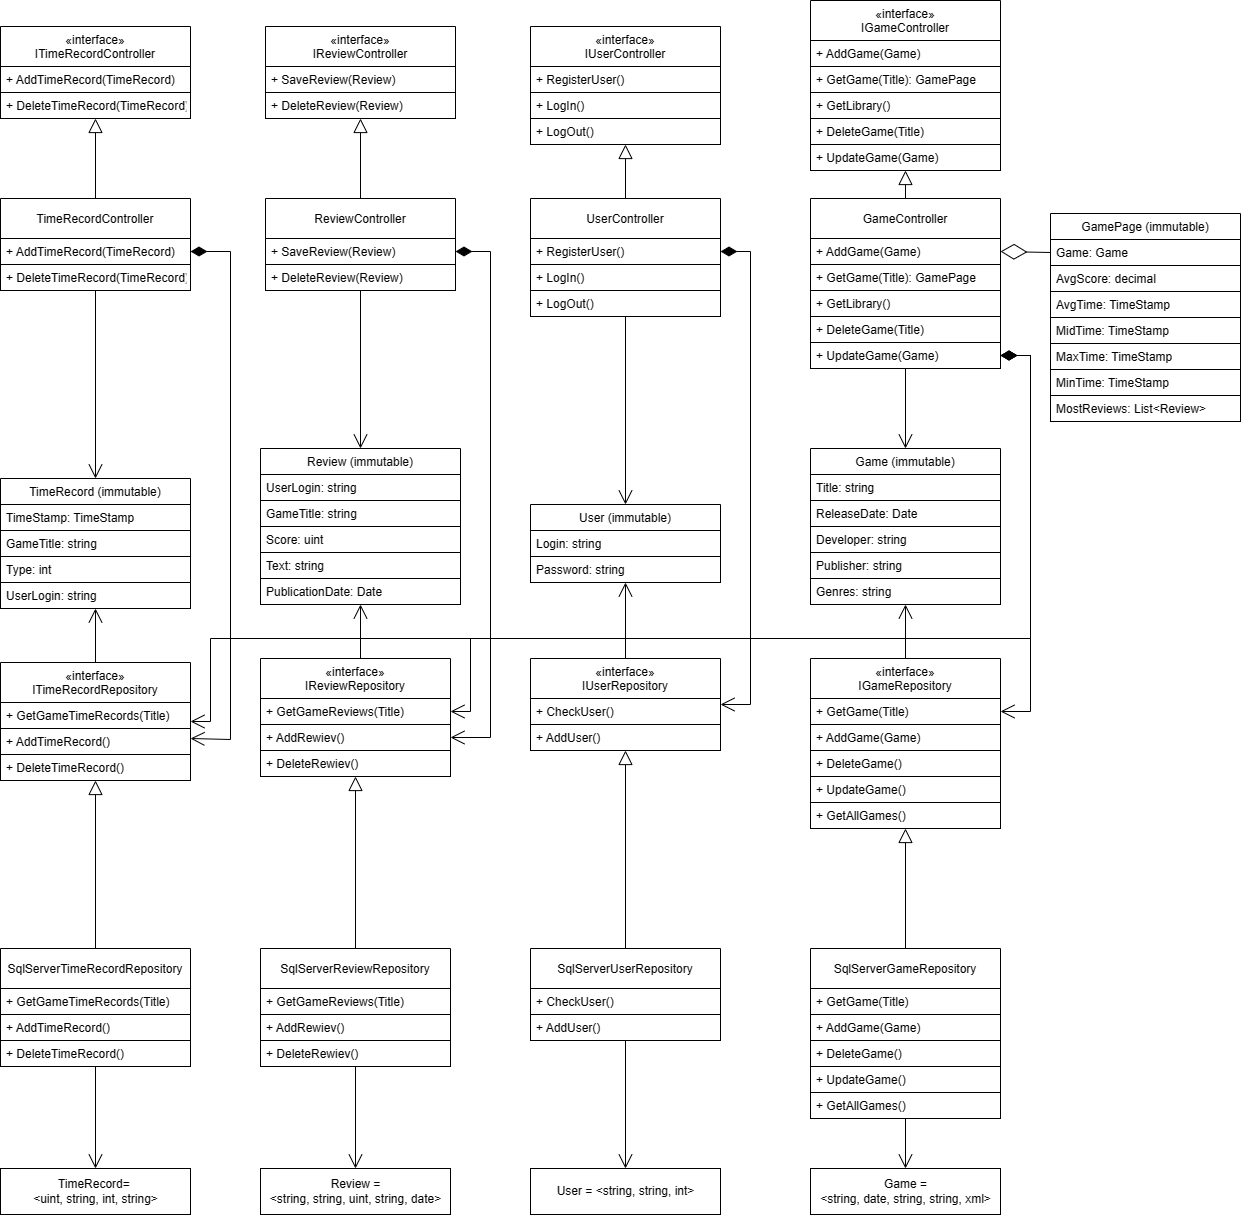
\includegraphics[width=1\linewidth]{../imgs/uml}
	\captionsetup{justification=centering}
	\caption{Диаграмма классов}
	\label{fig:uml}
\end{figure}

